\documentclass{standalone}
% \documentclass[preview]{standalone}
\usepackage[fontset=fandol]{ctex}
% 公式
\usepackage{amsmath}
% 公式符号加粗
% \usepackage{bm}
% TikZ 图形
\usepackage{tikz}
% 多图
\usepackage{subfigure}
% 插入三维图形
\usepackage{pgfplots}
\pgfplotsset{width=13cm,compat=1.18}

\begin{document}

\begin{figure}[t]
\centering
\subfigure[$x^2 + y^2 + z^2 \leq 1$]
{
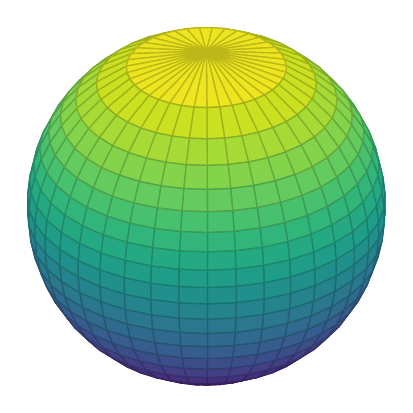
\begin{tikzpicture}[scale=1.2,transform shape]
\begin{axis}[
  hide axis,
  samples=20,
  samples y=40,
  domain=-1:1,
  y domain=0:2*pi,
  axis equal,
  colormap/viridis,
  z buffer=sort,
]
\addplot3 [surf]
(
  {sqrt(1 - x^2) * cos(deg(y))},
  {sqrt(1 - x^2) * sin(deg(y))},
  {x}
);
\end{axis}
\end{tikzpicture}
}
\subfigure[$x^2 + y^2 \leq z$]
{
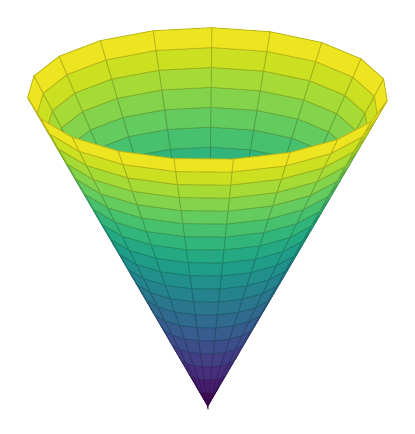
\begin{tikzpicture}[scale=0.8,transform shape]
\begin{axis}[
  hide axis,
  domain=0:1,
  y domain=0:2*pi,
  xmin=-1.5, xmax=1.5,
  ymin=-1.5, ymax=1.5, zmin=0.0,
  colormap/viridis,
  samples=20,
  samples y=20,
  z buffer=sort,
]
\addplot3 [surf]
  (
    {x*cos(deg(y))},
    {x*sin(deg(y))},
    {x}
  );
\end{axis}
\end{tikzpicture}
}
\subfigure[$\frac{x^2}{a^2} + \frac{y^2}{b^2} + \frac{z^2}{c^2} = 1$]
{
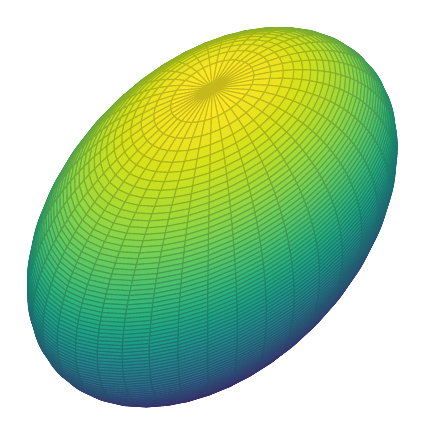
\begin{tikzpicture}
\begin{axis}[
  hide axis,
  axis equal,
  colormap/viridis,
  domain=0:2.00,
  samples=40, 
  z buffer=sort,
]
\addplot3 [surf,domain=-1:0,domain y=0:360] (
    {sin(y)*sqrt(1-x^2)},
    {2*cos(y)*sqrt(1-x^2)},
    {x}
  );
\addplot3 [surf,domain=0:1,domain y=0:360,on layer=axis foreground] (
    {sin(y)*sqrt(1-x^2)},
    {2*cos(y)*sqrt(1-x^2)},
    {x}
  );
\end{axis}
\end{tikzpicture}
}
\subfigure[$\frac{x^2}{a^2} + \frac{y^2}{b^2} = \frac{z^2}{c^2}$]
{
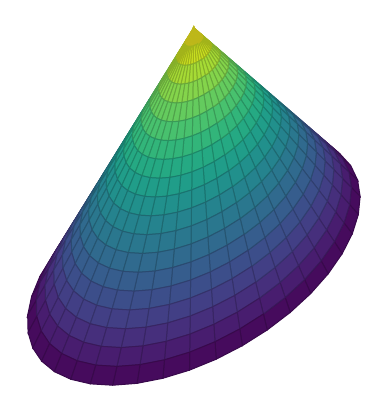
\begin{tikzpicture}[scale=0.9,transform shape]
\begin{axis}[
  hide axis,
  axis equal,
  colormap/viridis,
  domain=0:2*pi,
  samples=20, 
  samples y=40,
  z buffer=sort,
]
\addplot3 [surf,domain=0:2,domain y=0:2*pi] (
    {1*sin(deg(y))*(2-x)/2},
    {2*cos(deg(y))*(2-x)/2},
    {x}
  );
\end{axis}
\end{tikzpicture}
}

\caption{锥}
\label{fig:cone}
\end{figure}
\end{document}
